\documentclass[8pt,a4paper]{extarticle}
%\documentclass[8pt,twocolumn,a4paper]{extarticle}
%\documentclass[6pt,a4paper]{article}
\usepackage[utf8]{inputenc}
\usepackage{amsmath}
\usepackage{amsfonts}
\usepackage{amssymb}
\usepackage{graphicx}
\usepackage{enumitem}
\usepackage{setspace} 
\usepackage{float}
\usepackage{url}
\usepackage[usenames,dvipsnames,svgnames,table]{xcolor}
\usepackage{multicol}

\pagecolor{black}
\setlist{nolistsep}
\topmargin -2cm
\oddsidemargin -1.5cm
\evensidemargin -1.5cm
\textwidth 18.75cm
\textheight 26cm
\linespread{1.00}
\color{YellowOrange}

%Other Colors: ForestGreen,Cerulean,Salmon,Purple, Red, White

\twocolumn
\title{React and Redux Bootcamp:}
\author{Sean al-Baroudi}

\begin{document}

\newcommand{\mitem}{\item[$\square$]}
\newcommand{\mmitem}{\item[$\triangledown$]}

\maketitle


\section*{First React Application:}

\begin{itemize}
\item To start a React Project, most developers will utilize the create-react-app project template (a node package). Simply install this package and run it to start.
Specifically:

\begin{verbatim}

npx create-react-app <project name>
mkdir <project name>
npm start

\end{verbatim}

to install and get the local server running.

\item \textbf{Project Structure:}
\mitem \textbf{./nodemodules:} All locally installed node dependences are stored here.
\mitem \textbf{./public:} index.html (front page, robots.txt and favicons stored here.
\mitem \textbf{./src:} Contains the React Apps (self-contained pieces of interface+code), and support files, including:

- App.js (contains template React App)
- .test files (to run tests later)
- index.js: Where we Insert our App DOM object into the index.html DOM tree (at root).

\item The following minimial code is needed to insert our content into the index.html DOM tree:

\begin{verbatim}
import React from 'react';
import ReactDOM from "react-dom";
ReactDOM.render(<div>Our React Element </div>, 
document.getElementById("root"));
\end{verbatim}

\item In react, we typically bundle reusable UI elements into \textbf{Components}. 
\item \textbf{Components:} reusable pieces of React code to control part of the user interface. Components capture the structure of UI, and can have internal data to track the user behavior throughout the lifetime of the app.

\begin{verbatim}
import { Component } from 'react';
\end{verbatim}

\item Note that Classes, extended Sub-Classes and object Instances are used heavily in React - so be familiar with OOP.
\item A typical design pattern in React will be to extend template component classes, and add additional fields/methods to implement your application.
\item React automatically detects saved changes, and the local server updates. So you can update accordingly.
\item \textbf{State Field:} Subclasses of the Components class have a state field that we can use. We can link an object to this field, to maintain current state as the Component runs.
\item \textbf{State:} Dynamic data in a React component. This is often used to track variables that will be re-rendered in the UI based on events that occur in the application.
\item \textbf{React Rule:} \textbf{Never} Directly Modify the State property, if your intention is for changes to occur in the render method based on the updated state values. Use \textit{setState()} instead.
\item \textbf{But Why??} React is \textit{designed to re-render()} a given component when the setState() function is called. If you modify state directly, the changes will \textbf{not} be reflected in browser.
\item \textbf{Props:} Just stands for "Property". Data in a React component that gets passed down from its parent. In the parent component, it will pass data down to the child component through attributes in the child component’s JSX.
\item \textbf{How does the passing work?} See the example below:

\begin{verbatim}
class Profile extends Component {
 const {img, link} = this.props.profile

...

}

class SocialProfiles extends Component {
render() {
...
SOCIALPROFILES.map( prof => {
return )
<Profile key={prof.id} profile={prof />
...

}
}
\end{verbatim}

Note that the SOCIALPROFILEs data object gives us our data for this example. We map() on each element of the object.

Here, our Profile class defines a component that is a child to the SocialProfiles Class. We instantiate an object of the Profile class using the $<$Profile tag$>$. In the tag, we have placed properties (id, profile) that are fed into the object instance of Profile. We then can access these properties with \textit{this.props(.profile...)}
\item Visual Summary, \textbf{our modified \textit{create-react-app} project:}

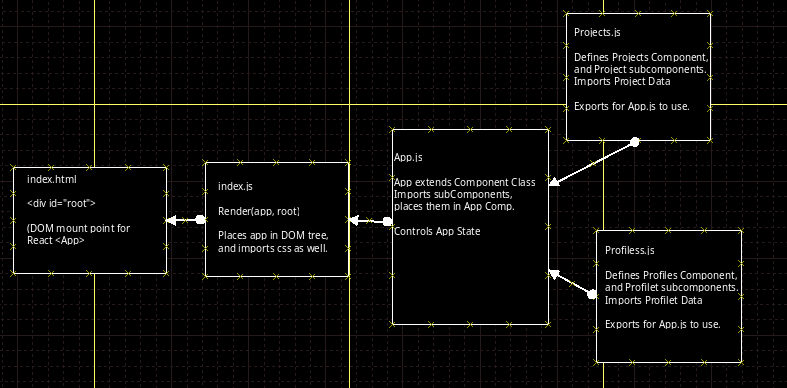
\includegraphics[scale=0.27]{appstructure.png}

\end{itemize}



\section*{Breaking Down React: React and Web Development:}

\begin{itemize}
\item Much of the structure in \textbf{create-react-app} is not necessary to get a minimal example to run.
\item All an app needs is one index.html page, and index.js page.
\item You don't even need to run "npm start" or "node react" - you can use CDNs to load React and ReactDOM libriaries straight into the browser.
\item \textbf{The Minimal Example is as follows:}
\mitem React CDN script tags at the end of index.html
\mitem A div root tag in index.html, so React can insert our $<$App$>$ into the DOM tree.

In index.js you can just build an app, render() and insert it as normal.
\item \textbf{JSX:} This is syntactic sugar that is transpiled to code that the browser will understand, when we run our react project (with npm start).
\item Transpilation is typically done with the \textbf{Babel package}.
\item \textbf{Why use Babel?} Javascript compliance is entirely Browser dependent - and JS core language development is completely separate from Browser development. When we want new features that Browsers may not yet support - we can transpile code to cruder JS so that it can be used in current browsers.

\item \textbf{Bundling and Transpiling:} Note that our React project will run in the browser, but ultimately Chrome/FF will not support our import/export system, nor will it support JSX. So we use a \textbf{bundler package (Parcel)} that utilizes Babel to produce a low-level enough JS file so that Chrome/FF can run our app. 
\item Parcel traces our application code, and finds all possible dependences, and then places all imported code into one mega-js file. Any syntactic sugar (such as JSX) is transpiled into lower level JS code that a browsre can understand.

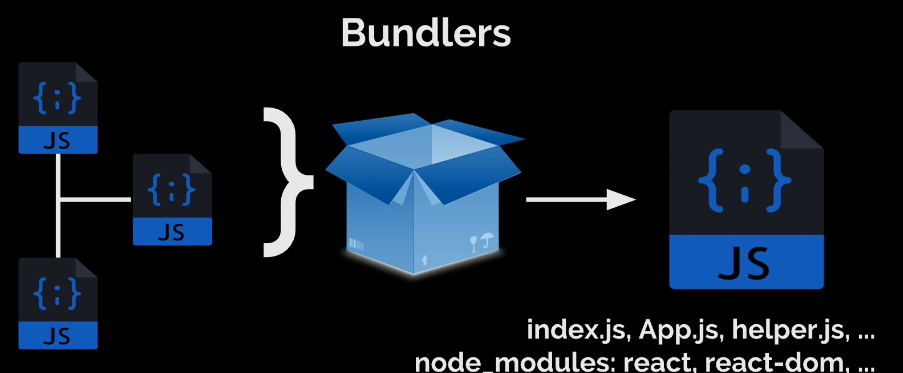
\includegraphics[scale=0.24]{bundle.png}

\item \textbf{Why Use Parcel?} The alternative is to import multiple scripts into the index.html page. These are loaded in order. As our project incrases in size+complexity we may deal with loading issues (namespace clobbering, circular dependencies, etc). To avoid this, Parcel will make one large JS file where dependency/NS issues are alleviated.

\item \textbf{Basic Parcel Usage:}

\begin{verbatim}
parcel <index.html>
\end{verbatim}

It will trace back all code depedencies from here.
 
\item \textbf{Parcel Folders (in project):} These will appear after you run parcel the first time:
\mitem \textbf{.cache}: Stores compiled elements to minimize recompilation later.
\mitem \textbf{dist:} Folder where bundled+transpiled JS code is stored - will rewrite index.html script links to point to this directory!
\item Using Parcel for Dev and Production: Parcel has a hot-wire feature - we can run it with the index.html, and it will auto-update all our code as we develop it.

Parcel however is heavier-weight - we don't use it when we launch produciton code. The following package.json scripts would be seen for a parcel build:

\begin{verbatim}
"scripts": {
    "dev": "parcel src/index.html",
    "build": "parcel build src/index.html",
    "start": "npm run build && live-server dist"
  }
\end{verbatim}

A lighter server (live-server) is chosen to strip down the size of the compiled production build, for launch.

\item \textbf{VirtualDOM:} React has its own stripped-down DOM model, so that it can make dynamic changes to the application page. Note: You don't use native DOM methods (like createElement, getElementById()...) in React - it has its own framework calls to do manipuations.
\end{itemize}

\section*{Continued Main React Concepts:}

\begin{itemize}
\item \textbf{Component Lifecycle:} Components have various event methods, that can be triggered during there operation. In particular, we are interested in when the component starts up, and when it shuts down with two methods:
\mitem \textbf{componentDidMount():} Called after component is loaded. If the method has to perform setup work or a fetch(), write this code in here.
\mitem \textbf{ComponentWillUnmount():} Called just before a Component is unmounted and destroyed. Use this as a takedown/cleanup
/signalling method.
\item Both methods above are written in the Component extended class - use non-first class functions only. "function" keyword is not required (its a JS class!).
\item \textbf{Stateless Functional Components:} Simplified Notation can be used, if our components contain no state. See Example Below:

\begin{verbatim}

const Project = props => {
	//destructure
  const { title, image, description, link } = props.project;
 
  return (
    <div style={{}}>
      <h3> {title} </h3>
      <img src={image} alt='profile' />
      <p>{description}</p>
      <a href={link}>{link}</a>
    </div>
  )
}
\end{verbatim}

Notice that for static/one-time components, we don't even need the render() method. We can even skip the return and encase the functional body with () - however we did destructuring above, so in this case it cannot be made that simple. Most simple example below:

\begin{verbatim}
const SimpleComp = props => {
	<div>   ~~SOME JSX~~   </div>
}
\end{verbatim}


\item \textbf{fetch():} Default Node/React method for making HTTP calls to external sources.
\item fetch() returns a JS Promise - and is an asyncronous function.
\item \textbf{Fetch Example 1:} Get a JSON object and print it:

\begin{verbatim}
fetch("http://localhost:3005/random_joke")
    .then(response => console.log(response.json()))
    .catch(error => console.log("Error:", error.message));
\end{verbatim}

Will print out json object to console. Basic errors also handled.

\item Example 2: Extract an array of JSON objects from promise, and work with them:

\begin{verbatim}
...
  state = {...jokes: []};

  fetchJokes = () => {
    fetch("http://localhost:3005/random_ten")
    .then(response => response.json())
    .then(json => this.setState({jokes:json}))

...

 { //At site where we want to print objects...
   this.state.jokes.map(joke => (
   <Joke key={joke.id} joke={joke}/>
    ))
 }
\end{verbatim}

We use the state and setState to pull the jokes array.

\item \textbf{Higher-order Components:} A higher-order component is one that takes another component as an input. The idea is to treat the component like a function. Have one component as input, and then output an entirely new component based on that input, with new properties, methods, and/or JSX!
\item
\end{itemize}

\section*{Music Master 2.0}

\begin{itemize}
\item API service was not available for this project, I just found my own data source instead and did my best. Some useful coding patterns/concepts are below:

\item \textbf{Arrow callbacks - Returning the Callback itself} (instead of return() value):

\begin{verbatim}
myfunction => props => () => { return(...)}
\end{verbatim}

This will return the inner function, with access to the outer parameters. In other words, equivalent to:

\begin{verbatim}
function (props) {
	return function() { body... }
}
\end{verbatim}
\item
\end{itemize}

\section*{Redux and more Advanced React:}

\begin{itemize}
\item Redux is a State Management technology.
\item It handles all the underlying data for your React application by enforcing a universal flow of data - that components can read from and add to using dispatchable actions.
\item It passes state/data between different components in our Application. 
\item Parent $\rightarrow$ Child data-passing can be prohibitive in complex situations - so we use Redux for a cleaner solution.
\item \textbf{Main Parts of Redux:}
\item 1) \textbf{(Global) Store:} Collects the state of the entire application.
\item 2) \textbf{Reduces:} Reducers split up the store and describe how sections of the store should update.
\item \textbf{Actions:} Objects (emitted events) full of data, processed by Reducers.
\item 4) \textbf{Dispatchers:} Components that create action objects.
\item This model creates a \textbf{Unidirectional Flow} of data.

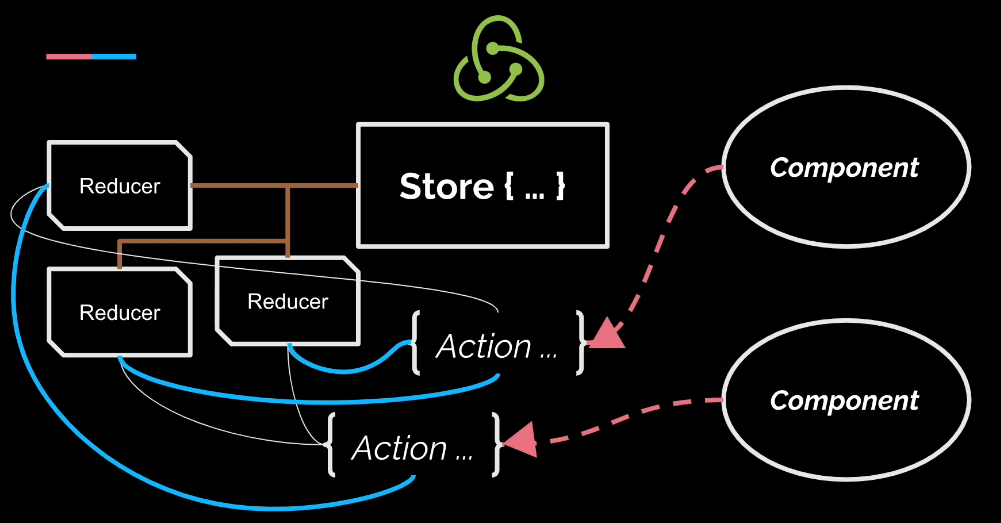
\includegraphics[scale=0.25]{redux_chart.png}

\item Actions are objects full of data that the reducers listen to. These actions are dispatchable by components. And reducers will then use the action data to update the redux store.
\item All reducers listen for actions (events that contain data). Each one fires, and checks the type of the action - to see if it handles it.
\item It is the responsibility of the programmer to check/filter types correctly in each reducer.
\item Actions are typed objects: they must contain a \textbf{type} field - this is how reducers filter them. An example of an action:

\begin{verbatim}

export const startGame = () => {
  return {type:SET_GAME_STARTED, gameStarted:true};
}

\end{verbatim}

\item Redux and React are two separate frameworks - they must be integrated together in a project. This specifically means: 
\item React Redux provides the connection between the redux system and the React components. Particularly: 
\mitem The Provider component wraps the App (in index.html) gives each component access to the Redux store.
\mitem The connect() function allows each component to customize what parts of the redux store it wants to read, and what actions the component should be able to dispatch.
\item 1) Components in React act as dispatchers for actions (Redux)
\item Components in React will query the Redux Global Store, to interpret application state.
\item \textbf{Redux Structuring:} The following folders and files are used, for each of the key objects in Redux:
\item 1) Actions: Stored in an $./src/actions$ folder. \\

There is a settings.js file where all arrow function actions are stored, and exported.\\

There is a types.js file, which lists all of our action types and exports them (so Reducers can use the types). An example of a type constant:

\begin{verbatim}

export const SET_GAME_STARTED = "SET_GAME_STARTED";

\end{verbatim}

\item 2) Reducers: Placed in the $./src/reducers$ folder, in a file called index.js. These are exported as well. An example of a reducer:

\begin{verbatim}

const rootReducer = (state = DEFAULT_SETTINGS, action) => {
 
  switch(action.type) { 
    case SET_GAME_STARTED:
      return {
        gameStarted:action.gameStarted,
        instructExp:state.instruct
      }; 
    case SET_INSTRUCTIONS_EXPANDED:       
    return { ...state, instructExp:action.instructExp };
    default:
      return state;
  }
}

\end{verbatim}

\item 3) Dispatching Setup: This is typically done in App.js. See the following code:

\begin{verbatim}
import React, { Component } from 'react';
import { connect } form 'react-redux';

class App extends Component {
  render() {
    return (
      <div>React App</div>
    );
  }
}

const componentConnector = connect();

export default App;
\end{verbatim}

The connect() function connects the App component to Redux, so it can be used as a dispatcher.

\item \textbf{MapStateToProps}: The first argument to the connect function. Allows you to specify what data the component should have from the redux store. You map the redux store state to the props object of the component.

\item \textbf{MapDispatchToProps}: The second argument to the connect function. Allows you to specify what methods should be made available to the component (through props), that will be able to dispatch the results of action creators to the store.



\item 4) Setting up the Provider Frame: Note that to use global state, we must wrap our App in another structure called a Provider. We do this in the project index.js file:

\begin{verbatim}
import React from 'react';
import ReactDOM from 'react-dom';
import App from './components/App';
import { createStore } from 'redux';
import { Provider } from 'react-redux'; 
import rootReducer from './reducers';

const store = createStore(rootReducer);

ReactDOM.render(
  <Provider store={store}>
    <App />
  </Provider>, document.getElementById('root'));

\end{verbatim}


\item Reducer Debug Tip: Instead of internal console.log() statements, use the subscribe() function:

\begin{verbatim}

store.subscribe(() => console.log("store.getState()",store.getState()));

\end{verbatim}

\item Redux Middleware code runs in between the point that an action gets dispatched and the reducers receive the action objects. Think of it as extensions for the redux system; it’s useful for adding new capabilities to the underlying redux logic. One such middleware is redux-thunk.

\item Redux \textbf{thunk} is a library that allows for asynchronous actions to be dispatched. Normally, actions are plain objects. But in the case of using the fetch method, to make an api call, an asynchronous action is useful in order to dispatch different kinds of actions based on the result of the api call.

\item LocalStorage is a JavaScript object that can be used to store items in a key-value structure within the browser.

\item \textbf{Dealing with Cross Origin Resource Sharing:} When making a fetch() request to a remote server, the request will often fail because of the CORS policy. 
\item \textbf{What is CORS?}
\item \textbf{Definitions (for CORS):}
\mitem origin: the server the application is running from.
\mitem (an) origin: the source of a particular resource.
\mitem permitted origin: a sourced allowed by the browser to serve content - it lives outside the application itself.
\mitem cross-origin: when the providre and destination of a resource do not match.
\item Simple Request: One defined as a GET/HEAD/POST method with safe header fields. See \cite{cors} for details.
\item Same Origin Policy (Summary): A web application using XMLHttpRequest and Fetch() can only request resources from the same origin the application was loaded from unless the response from other origins includes the \textbf{right CORS headers}.
\item CORS only applies to HTTP requests to external sources, from scripts. This is to suppress unwanted requests from hijacked applications.
\item \textbf{Different Header Options:}
\item \textit{External Server:} the Header option for CORS is \textit{Access-Control-Allow-Origin} - this is set in the response object from the external source. If set to "*", any application can request resources from the server. For better security settings - a resource provider will have a short-list of approved applicatoins.
\item \textit{App Origin:} For a non-simple request (not a simple GET/POST...), a preflight request is sent to the external server by the browser. This consists of an OPTIONS request with the \textit{Access-Control-Reqest-Method} and \textit{Access-Control-Request-Headers} fields set. Once the response is sent back and is approved by browser, the non-simple request is sent out.

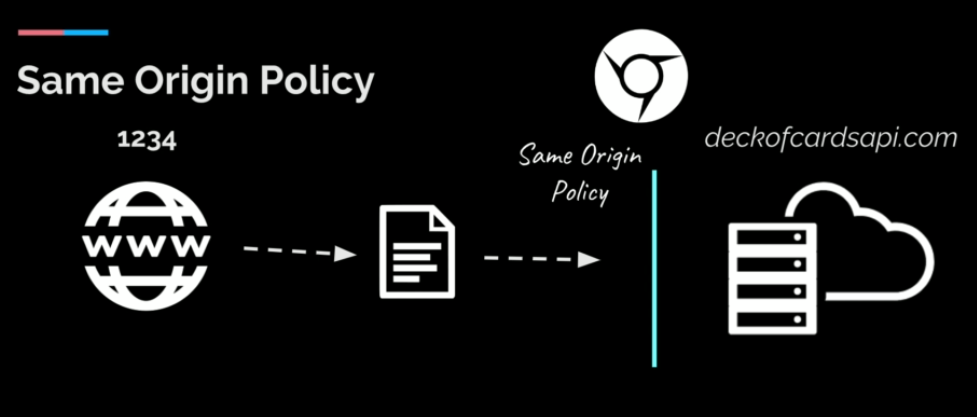
\includegraphics[scale=0.22]{cors.png}



 
\end{itemize}

\section*{Redux Project: Reaction:}
\begin{itemize}
\item For this applicaiton, we will implement the Publisher-Subscriber Architecture for our app, to allow subscribers to a channel to post messages, and reply with Emoji's.
\item Pub/Sub: A software pattern that allows publishers to send information to channels that subscribers will listen to. A good networking option that can reduce the usual approach of keeping a list of all addresses that are connected to the network.
\item We will have multiple instances of the application running. Redux Data Flow is structured as follows:

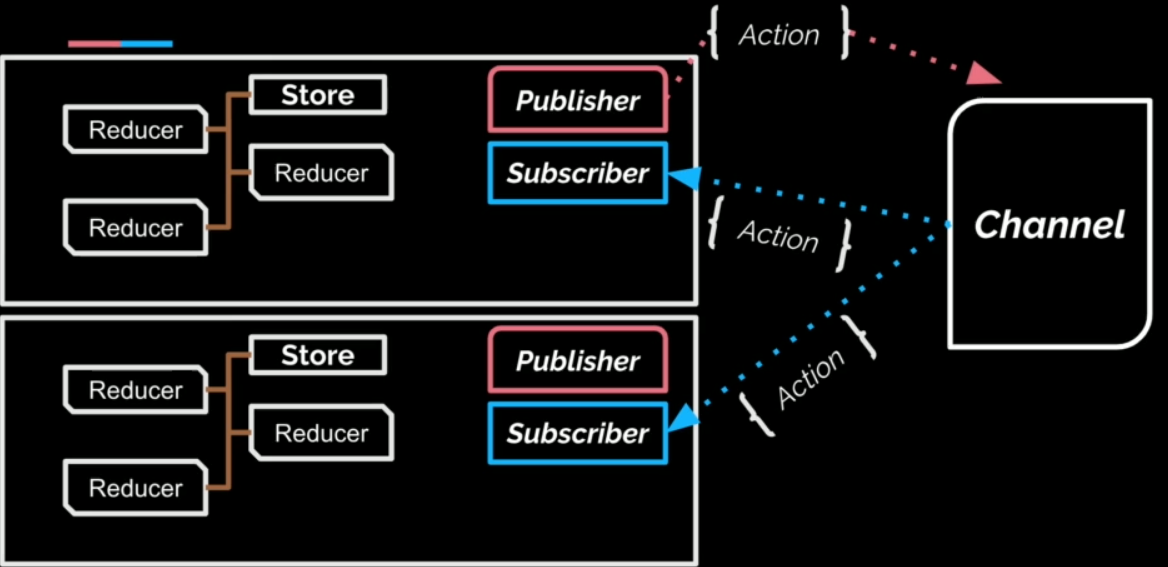
\includegraphics[scale=0.20]{pubsub.png}

\item The steps our application will take, to send a message, are as follows:
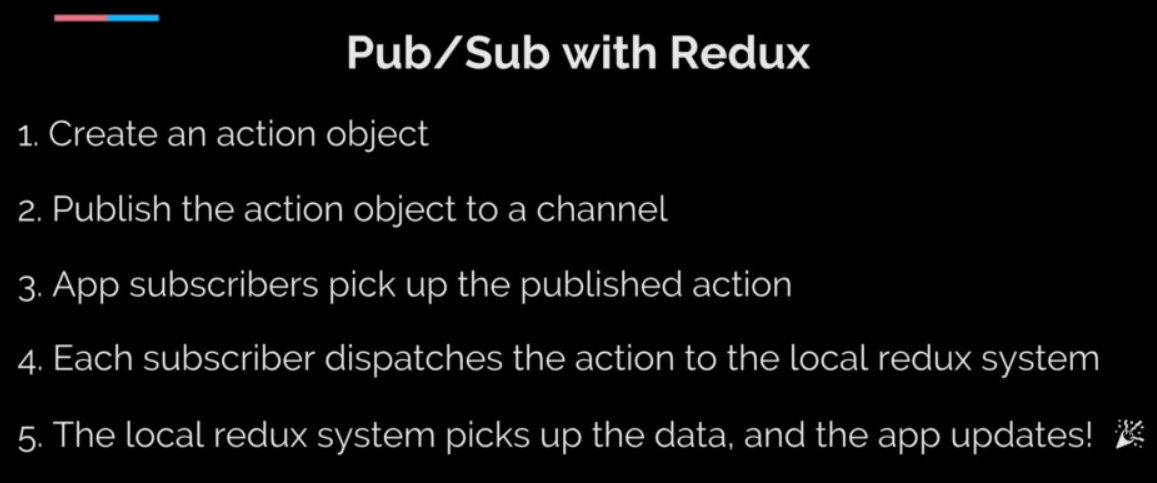
\includegraphics[scale=0.20]{pubsublist.png}

\item \textbf{React Context:} A way to share data between many React components without having to pass that data down manually through props. A component will look to the nearest parent component, that is a context Provider, to get the values that it can use for its own component `context` field.
\item The Context Provider Component uses a value property to provide data to any nested component through its context field.
\item The Redux devtools is an extension that allows you to examine the redux store state, and see actions being dispatched in real time.
\item
\item Connecting to React DevTools: Download app in Chromium, and use the folloiwng createStore() arguments:

\begin{verbatim}

const store = createStore(rootReducer,window.__REDUX
_DEVTOOLS_EXTENSION__ && window.__REDUX_DEVTOOLS_EXTENSION__());

\end{verbatim}
\item A diagram of our project is as follows:

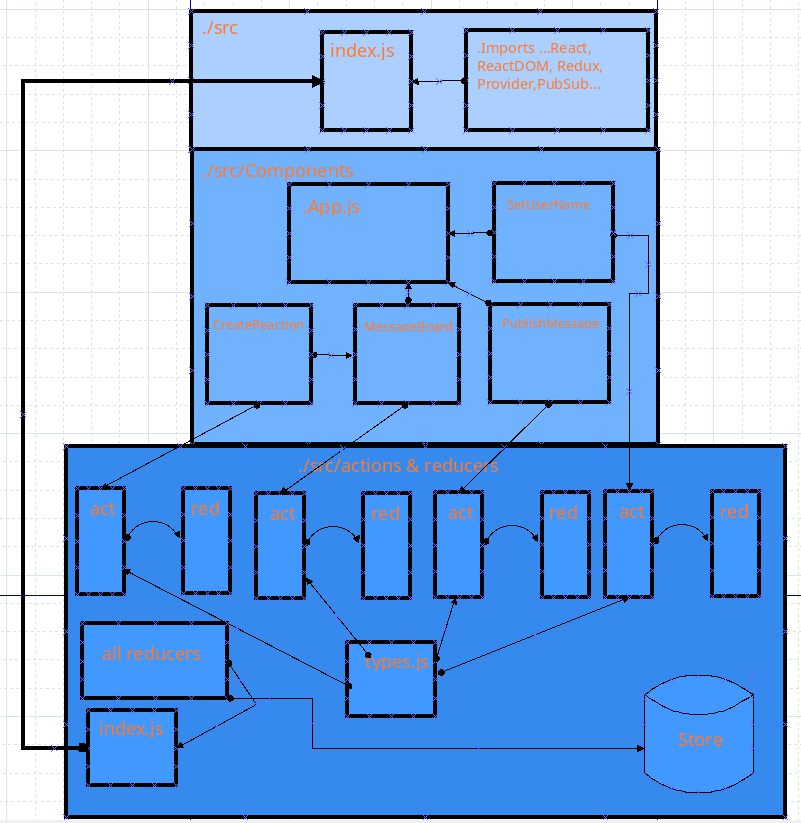
\includegraphics[scale=0.3]{reaction_flowdiagram.png}


\end{itemize}



\section*{Create Backend APIs for React Apps:}
\begin{itemize}
\item Express is a framework built on top of Node.js used for starting servers and building web APIs.
\item Express middleware is functionality that runs before every request, to process information about the request, add headers to the response, perform logging, and any other kind of useful functionality. Code Examples Below:

\begin{verbatim}

app.use((req, res, next) => {
  res.header("Access-Control-Allow-Origin", "*");
  next();
})

\end{verbatim}

These middleware modules act as listeners that are fired before GET() listeners are engaged. the Next() method allows us to continue processing in other middleware listeners. The RES() object allows us to respond to the client prematurely.
\item Our express can serve requests with the get() method:

\begin{verbatim}
app.get('/ping', (req,res) => {
  res.send('pong')
});

app.get("/stories", (req, res) => {
  res.json(stories);
});
\end{verbatim}

Note: Avoid appending paths with "." (Linux Habit). Error 404 will occur!


\item \textbf{CORS policy for API:} Adding the `Access-Control-Allow-Origin` with the `*` argument will allow any frontend addresses to be considered as part of the server’s origin. This helps get past the same origin policy check implemented by the browser.
\item API Wrappers are servers that perform inner requests to other APIs. These can be used to combine multiple API requests into one overall request, to add a more open `Access-Control-Allow-Origin` header, and to accomplish other custom functionality!
\item Serving a React Frontend can occur within the same server as its backend API. Serve a static directory to the relative path where your React code is built.
\item To do this, we merge our client and api projects. This involves splicing the package.json file of the client project into the package.json of our express project. See git directory for details. Run npm i to install all packages in the root directory.
\item We can get our API to serve front end files with the following code:

\begin{verbatim}
const path = require("path");

...

app.use(express.static(path.join(
__dirname, "client/dist")));
\end{verbatim}
\item \textbf{Why does this work?}

Because the index.html file of the react app has been put in client/dist by parcel running in the background. Note our modified npm start script:

\begin{verbatim}
    "start": "npm run build-client && node ./",
\end{verbatim}

As long as the paths dont' clobber, we can access React content and our API with the same localhost:3000 domain!

\item \textbf{Caveat:} If we do this, dynamic page loading is disabled. If we want to develop our API and React App, and see the front end update on saves, we can run:

\begin{verbatim}
Tab1: npm run dev
Tab2: npm run dev-client
\end{verbatim}
\item
\end{itemize}

\section*{Deployment of our App (Heroku):}

\begin{itemize}
\item \textbf{Steps for launching a Heroku App:}

\item 000) Sign up for Heroku, setup 2FA, install on your desktop.

\item 00) Run *heroku login* on command line, and connect.

\item 0) Make sure this project is uploaded to its own github repository before you start.

\item 1) Now Adjustments to our App need to be done:

\item a) Adjust the fetch() URL from \textit{"localhost:3000..."} to \textit{`$\{$document.location.origin$\}$`}.

\item   b) Add an environment generated port number to index.js: with \textit{const PORT = process.env.PORT $\vert \vert$ 3001;}

\item 2) Once changes are complete, commit changes to github repository one more time.

\item 3) Run \textit{git push heroku main} to run the application in the cloud.

\item 4) (Optional): See the Heroku setting panel to adjust port/url/mapping etc. Remember to update the github repo link if you make this change with:  \textit{git remote set-url $<$new heroku url$>$}

\item
\end{itemize}


\begin{thebibliography}{9}

\bibitem{cors}
\url{https://developer.mozilla.org/en-US/docs/Web/HTTP/CORS}	
\end{thebibliography}


\end{document}
